\chapter{Real Estate Leverage, Deal Flow, and the Brokerage Machine}

This chapter follows a School of Hard Knocks entrepreneurship interview, curated by LazyingArt LLC through Video2Book, as a practical lecture on real estate wealth building. There is no blackboard in this source. The mathematics is the mathematics of commercial control: a small amount of cash controls a larger asset, a brokerage platform turns agents into deal sources, and media turns one conversation into a much larger audience. We will keep the transcript's rhythm: first the leverage claim, then the office tour, then the operating culture, then the machinery that produces leads and deals.

\section{Leverage Begins With Below-Value Buying}

The interview opens with a direct question: how many properties are owned right now? The answer is the proof point: right around \(130\) different properties after \(13\) years in real estate. The next question is not abstract. If someone is starting in real estate, what is the best advice?

The answer is compact: take the risk, but find properties that are below value. That qualification matters. Risk by itself is not the mechanism. The speaker is describing risk attached to an asset purchased at a discount to perceived value. In symbols, if \(P_{\mathrm{buy}}\) is the purchase price and \(P_{\mathrm{value}}\) is the buyer's estimate of fair value, the intended inequality is

\begin{equation}
P_{\mathrm{buy}} < P_{\mathrm{value}}.
\end{equation}

The transcript does not define how that value is measured. It could come from comparables, rents, redevelopment potential, land value, or a buyer already in view. The note we should keep is narrower and stronger: the deal begins only when the buyer believes there is a spread between price and value.

Then the speaker gives the numerical example that anchors the whole opening. Suppose a buyer puts down \(\$10{,}000\) on a property worth \(\$300{,}000\). If the property rises \(10\%\), the asset-level gain is

\begin{equation}
\Delta P = 0.10 \times \$300{,}000 = \$30{,}000.
\end{equation}

The point is not that the buyer owned the whole property free and clear. The point is that the buyer's initial cash controlled a much larger asset.

\subsection{Question \& Answer}

How can a \(10\%\) gain in the property become a claim that the buyer ``tripled'' the money?

The calculation compares the asset gain with the initial cash down payment:

\begin{equation}
\frac{\Delta P}{E_0}
=
\frac{\$30{,}000}{\$10{,}000}
=
3,
\end{equation}

where \(E_0\) is the initial equity or cash down payment. In this limited sense, the paper gain is three times the original cash. If the debt balance is unchanged and all costs are ignored, the paper equity position would be

\begin{equation}
E_1 = E_0 + \Delta P = \$10{,}000 + \$30{,}000 = \$40{,}000.
\end{equation}

So the phrase ``tripled your money'' should be read carefully. The transcript supports the statement that the gain is three times the cash down. It does not include interest, taxes, repairs, insurance, vacancy, closing costs, selling costs, or debt amortization. The speaker immediately adds the right caveat: it is on paper, and one has to think long term.

\begin{figure}
\centering
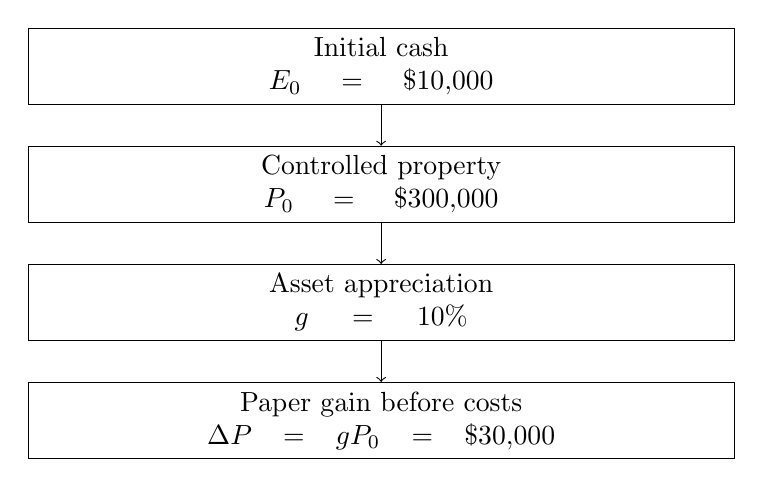
\begin{tikzpicture}
\node[draw, align=center, text width=0.72\linewidth] (cash) at (0,0) {Initial cash\\ \(E_0=\$10{,}000\)};
\node[draw, align=center, text width=0.72\linewidth] (asset) at (0,-1.5) {Controlled property\\ \(P_0=\$300{,}000\)};
\node[draw, align=center, text width=0.72\linewidth] (gain) at (0,-3.0) {Asset appreciation\\ \(g=10\%\)};
\node[draw, align=center, text width=0.72\linewidth] (paper) at (0,-4.5) {Paper gain before costs\\ \(\Delta P=gP_0=\$30{,}000\)};
\draw[->] (cash) -- (asset);
\draw[->] (asset) -- (gain);
\draw[->] (gain) -- (paper);
\end{tikzpicture}
\caption{The transcript's leverage example: a small cash position controls a larger asset, so an asset-level gain can be large relative to the cash down payment.}
\end{figure}

\section{Time Turns a Deal Into an Asset Base}

After the leverage example, the speaker widens the time scale. He recalls a person who bought a property for \(\$11{,}000\) and, roughly \(60\) years later, had an offer for \(\$3{,}000{,}000\). This is an anecdote, not a promised return. Still, it gives a useful comparison:

\begin{equation}
M
=
\frac{\$3{,}000{,}000}{\$11{,}000}
\approx
272.7.
\end{equation}

If we annualize that multiple only as a reconstruction, not as a stated claim, the implied annual growth rate would solve

\begin{equation}
1+r
=
\left(\frac{3{,}000{,}000}{11{,}000}\right)^{1/60},
\qquad
r \approx 9.8\%.
\end{equation}

This calculation should remain subordinate to the narrative point. The speaker is not teaching a compounding formula. He is making a long-horizon claim: real estate can reward patience because the asset has continuing use value. He then says that a house is not going to zero in the way a stock or a business might.

That statement should be preserved as a practical claim, not a theorem. A parcel or building may retain some residual value, but a specific investment can still be damaged by bad financing, vacancy, legal trouble, taxes, repairs, overpayment, or poor local demand. The chapter's mechanism is therefore not ``real estate cannot fail.'' It is more disciplined: buy below value, control the asset with appropriate leverage, and allow time to work while surviving the costs of ownership.

\section{The Brokerage as Shared Infrastructure}

The interview then pivots from the opening lesson to a tour. That movement matters. We are no longer hearing merely what the owners believe; we are being shown the infrastructure they use to make the belief operational.

The office is described as open to everyone. Agents can come work, throw events, hold parties, and use the space. The firm has moved into a newer Austin office while still keeping a Round Rock office. The building is rented, but the speakers say they have a first right of refusal to buy it. In commercial terms, this is a form of optionality: if another offer appears, they get the opportunity to buy.

The office tour also introduces training rooms and classes. The transcript says there is basically a class every day that month. In these notes, the office should be read as a platform:

\begin{equation}
\text{space} + \text{training} + \text{access} + \text{relationships}
\longrightarrow
\text{deal flow}.
\end{equation}

This is not an equation in the physical sense; it is an operating identity. A brokerage is not only a place where commissions are split. In the model described here, it is a place where agents are trained, deals are surfaced, and ownership opportunities are shared.

\section{From Commissions to Partnership and Equity}

The next major question is about process. How do agents move from commissions into partnering with the brokerage on deals? The speaker's answer begins with a phrase that repeats the chapter's deepest motif: finding value.

He says an agent does not need to make commissions for two years and then buy real estate with the brokerage. If the agent finds an opportunity now, the brokerage can buy it with them, show them how to do it, give them equity, create a new entity, and then build a portfolio.

\subsection{Question \& Answer}

What happens when an agent can see value but does not yet have the capital, partners, or experience to take the deal down?

The speaker gives the answer by recalling his own obstacle. When he was \(24\), he could see value in a property but could not buy it because his broker did not do commercial real estate. Looking back, he says he could have raised capital or brought on partners, but he did not know that when he was starting.

The brokerage is presented as the missing structure. The mechanism is not simply encouragement. It is a sequence:

\begin{figure}
\centering
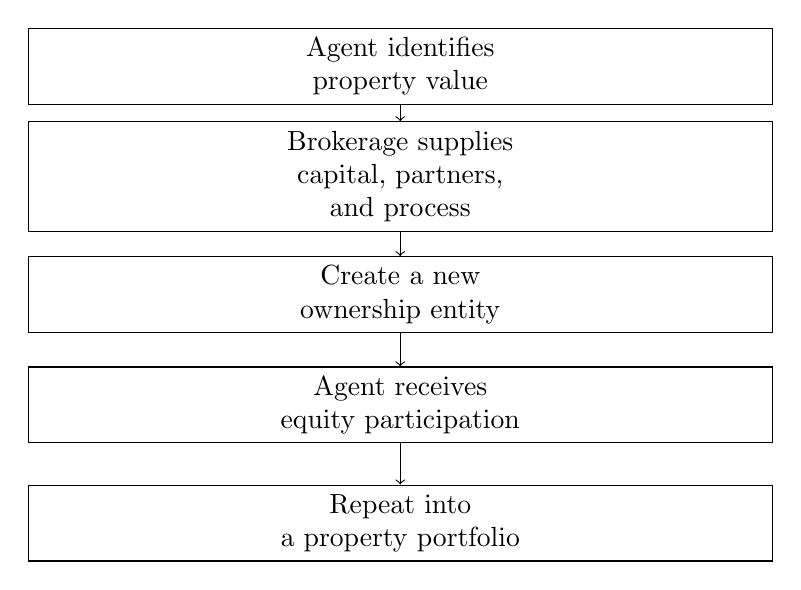
\begin{tikzpicture}
\node[draw, align=center, text width=0.76\linewidth] (agent) at (0,0) {Agent identifies\\ property value};
\node[draw, align=center, text width=0.76\linewidth] (support) at (0,-1.4) {Brokerage supplies\\ capital, partners,\\ and process};
\node[draw, align=center, text width=0.76\linewidth] (entity) at (0,-2.9) {Create a new\\ ownership entity};
\node[draw, align=center, text width=0.76\linewidth] (equity) at (0,-4.3) {Agent receives\\ equity participation};
\node[draw, align=center, text width=0.76\linewidth] (portfolio) at (0,-5.8) {Repeat into\\ a property portfolio};
\draw[->] (agent) -- (support);
\draw[->] (support) -- (entity);
\draw[->] (entity) -- (equity);
\draw[->] (equity) -- (portfolio);
\end{tikzpicture}
\caption{A transcript-backed reconstruction of the agent partnership model: the broker is not only a commission collector but a partner in turning found value into owned equity.}
\end{figure}

This is the lecture's second kind of leverage. The first was financial leverage: cash controls property. The second is institutional leverage: a platform lets a novice act on a deal that would otherwise exceed their capital or experience.

\section{Culture, Sales, and the Real Cost of Ownership}

The interview then asks what separates this brokerage from more corporate or cutthroat brokerages. The response is cultural but still operational. Most brokerages, in the speaker's framing, push agents to produce more commissions. This firm asks what the agent is really trying to do and how the firm can support it.

The menu is broad: build a brand, build a team, wholesale, buy real estate, or make commissions. The license is treated as one tool among several, not the whole business. The chapter should preserve that distinction. A real estate license can produce transaction income, but the larger aim described here is generational wealth through ownership and entrepreneurial optionality.

The next room introduces Killer Kim, who is doing cold calls. Asked for her secret to sales, she says she tries to be authentic. She loves talking to people and does not perform a false character. The lecture places this human sales note beside a harder ownership note. She owns \(16\) or \(17\) properties, has all but three paid off, and the conversation suggests about \(\$19{,}000\) a month.

But the transcript immediately resists the fantasy that property count alone means passive ease. There are foundation problems, septic problems, roofing problems, and continuous work. So the operating reality can be summarized as

\begin{align}
\text{rental ownership}
&=
\text{asset base}
+
\text{cash flow}
-
\text{repairs}
-
\text{debt service}
-
\text{management burden}.
\end{align}

This is not pessimism. It is the adult version of the opening leverage lesson. Leverage can amplify gains, but ownership also amplifies responsibility.

\section{Media as Message Leverage}

After cold calling and property operations, the interview turns to marketing. The firm is building a room where agents can go live on Instagram, TikTok, Facebook, and YouTube. The stated purpose is not just to look modern. It is to let agents record their own content and make the message personal.

The marketing team says that social media is one of the most valuable things the firm does. One person contrasts the scale of a live class with online distribution: a class might reach \(10\) people, while a social post can reach hundreds of thousands or millions. Later, in the podcast room, the aspiration is stated even more sharply: instead of talking to \(10\) people, talk to \(10\) million.

The same structure as financial leverage appears again. Let \(A_{\mathrm{room}}\) be the number of people reached in a room and \(A_{\mathrm{social}}\) the number reached online. The reach multiple is

\begin{equation}
M_{\mathrm{reach}}
=
\frac{A_{\mathrm{social}}}{A_{\mathrm{room}}}.
\end{equation}

If a live class reaches \(A_{\mathrm{room}}=10\) people and a piece of content reaches \(A_{\mathrm{social}}=100{,}000\), then

\begin{equation}
M_{\mathrm{reach}}
=
\frac{100{,}000}{10}
=
10{,}000.
\end{equation}

Again, this is not revenue by itself. Reach is not the same as trust, conversion, profit, or deal flow. But the speaker's point is credible as a mechanism: a message that can travel beyond the room changes the size of the opportunity surface.

\begin{figure}
\centering
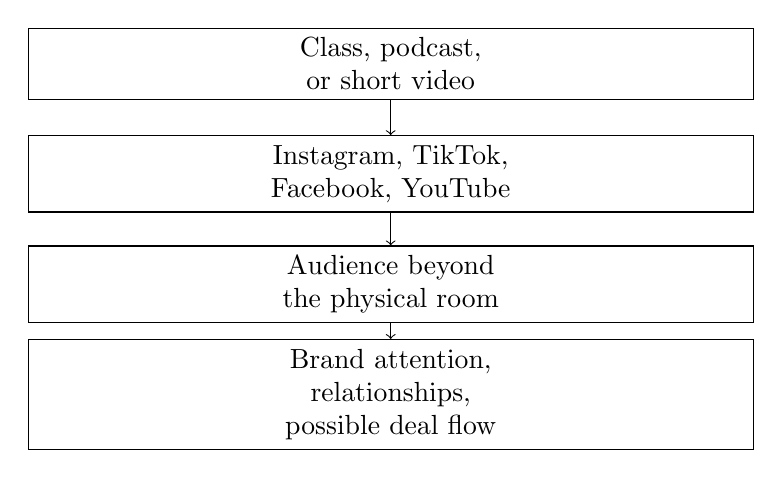
\begin{tikzpicture}
\node[draw, align=center, text width=0.74\linewidth] (class) at (0,0) {Class, podcast,\\ or short video};
\node[draw, align=center, text width=0.74\linewidth] (platforms) at (0,-1.4) {Instagram, TikTok,\\ Facebook, YouTube};
\node[draw, align=center, text width=0.74\linewidth] (audience) at (0,-2.8) {Audience beyond\\ the physical room};
\node[draw, align=center, text width=0.74\linewidth] (flow) at (0,-4.2) {Brand attention,\\ relationships,\\ possible deal flow};
\draw[->] (class) -- (platforms);
\draw[->] (platforms) -- (audience);
\draw[->] (audience) -- (flow);
\end{tikzpicture}
\caption{Media leverage in the lecture: one message is packaged so it can travel through platforms and reach an audience far larger than the room.}
\end{figure}

The Grant podcast story illustrates the same idea in narrative form. A late-night Clubhouse opening becomes an email, the email becomes a podcast booking, and the podcast becomes a business meeting. The lesson is not merely ``be persistent.'' It is that media access, preparation, and a clear agenda can convert attention into relationship capital.

\section{Finding Value, Wholesaling Land, and the Machine}

The final instructional movement returns to the most portable skill: learn how to find value and find deals. A five-year real estate operator says that whether one is an agent, wholesaler, investor, or capital raiser, the common skill is the ability to identify value and opportunity in any market condition.

Asked what he would do if he started from zero and had one year to make a million dollars, he answers: wholesale land in Austin, Texas. The process he describes is simple enough to write as a deal-spread model. Put land under contract at a good price, then find a developer or end buyer willing to pay more.

Let \(P_{\mathrm{contract}}\) be the contract price and \(P_{\mathrm{end}}\) the end-buyer price. The gross spread is

\begin{equation}
S_{\mathrm{gross}}
=
P_{\mathrm{end}} - P_{\mathrm{contract}}.
\end{equation}

For the method to be meaningful,

\begin{equation}
P_{\mathrm{end}} > P_{\mathrm{contract}}.
\end{equation}

That inequality is the wholesaler's version of buying below value. The person may not intend to hold the asset for decades; the value is in controlling a contract that another buyer values more highly. The transcript does not give specific numbers, so the chapter should not invent them. The important structure is the spread.

The tour then moves to Round Rock, where the speakers describe ``the machine.'' This is the call-center and lead-generation side of the brokerage. They do inbound and outbound work, reach out to people asking about homes, connect them with agents, and help route them through credit repair if needed, lending partners, and financing.

\begin{figure}
\centering
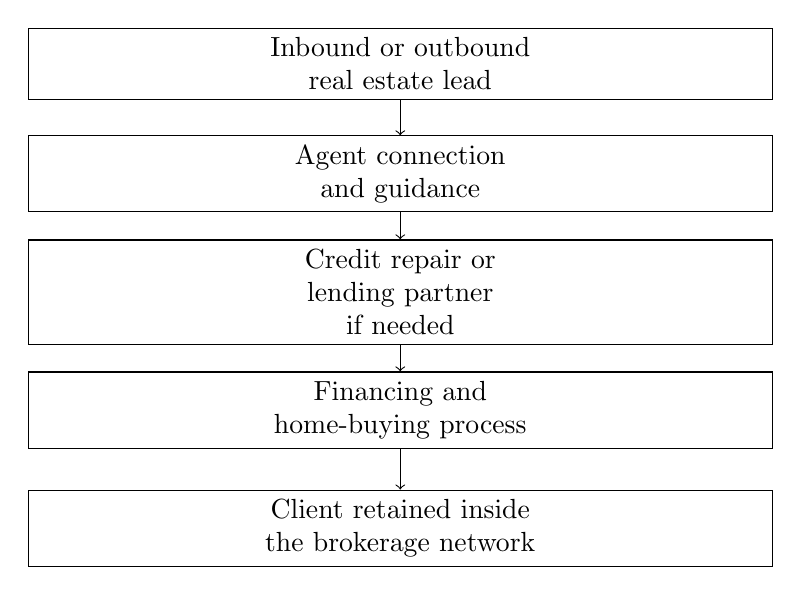
\begin{tikzpicture}
\node[draw, align=center, text width=0.76\linewidth] (lead) at (0,0) {Inbound or outbound\\ real estate lead};
\node[draw, align=center, text width=0.76\linewidth] (agent) at (0,-1.4) {Agent connection\\ and guidance};
\node[draw, align=center, text width=0.76\linewidth] (support) at (0,-2.9) {Credit repair or\\ lending partner\\ if needed};
\node[draw, align=center, text width=0.76\linewidth] (finance) at (0,-4.4) {Financing and\\ home-buying process};
\node[draw, align=center, text width=0.76\linewidth] (house) at (0,-5.9) {Client retained inside\\ the brokerage network};
\draw[->] (lead) -- (agent);
\draw[->] (agent) -- (support);
\draw[->] (support) -- (finance);
\draw[->] (finance) -- (house);
\end{tikzpicture}
\caption{The ``machine'' as described in the transcript: lead generation, routing, partner support, and an in-house client path.}
\end{figure}

This is the third form of leverage. We have seen financial leverage, media leverage, and now process leverage. A brokerage that repeatedly creates leads, assigns agents, and routes clients through trusted partners is no longer relying only on individual hustle. It is building a repeatable path.

\section{Summary}

The lecture begins with a simple real estate arithmetic problem and ends with an operating system. The opening example shows why leverage matters:

\[
R_E = \frac{gP_0}{E_0},
\]

but the transcript insists that this return is only paper until time, costs, debt, and execution are accounted for. The long-term property anecdote supplies patience; the office tour supplies infrastructure; the agent partnership model supplies a way for beginners to act on value; the cold-calling segment supplies human sales discipline; the media studio supplies audience leverage; and the Round Rock machine supplies process leverage.

The durable lesson is not that real estate automatically creates wealth. The lesson is that wealth is built when several forms of leverage are made to work together: buying below value, controlling assets with disciplined equity, sharing infrastructure with agents, distributing the message through media, and building systems that create and route opportunity.